\subsection{Module Interconnection}

By interconnecting the modules derived in the last chapter, datapaths are created. By forming cycles in the datapaths, the outputs of previous operations can be used as an input to new ones. The datapaths can also be multiplexed, i.e an output can dynamically be configured to be drive by one of multiple inputs. By doing so, the machine can execute different operations using identical hardware, depending on the configuration of the datapath. In this chapter, the datapath of the logical design is developed.

Initially, all modules derived in the previous chapter are free-standing, i.e they are not connected with each other in any way. The initial pieces of data needed to setup the execution of any one instruction is the instruction itself. More precisely, its binary representation and the individual fields within it, as explained in \autoref{sec:implementation_instruction_encoding}. The opcode field is used by the control unit to derive the relevant control signals. The three register fields of the instruction are passed to the register bank, while the immediate operand is passed to the \ac{alu} for computation. To select the current instruction, the program counter is read and used as an index for the program memory. \autoref{fig:implementation_interconnection_datapath_instruction_decoding} shows the relevant modules and the datapath after adding these connections. This set of modules and connections represents everything needed for the decode phase of the instruction cycle. As soon as the program counter is modified, the indexed instruction, and therefore all connected signals change their value.

\begin{figure}[h!]
    \centering
    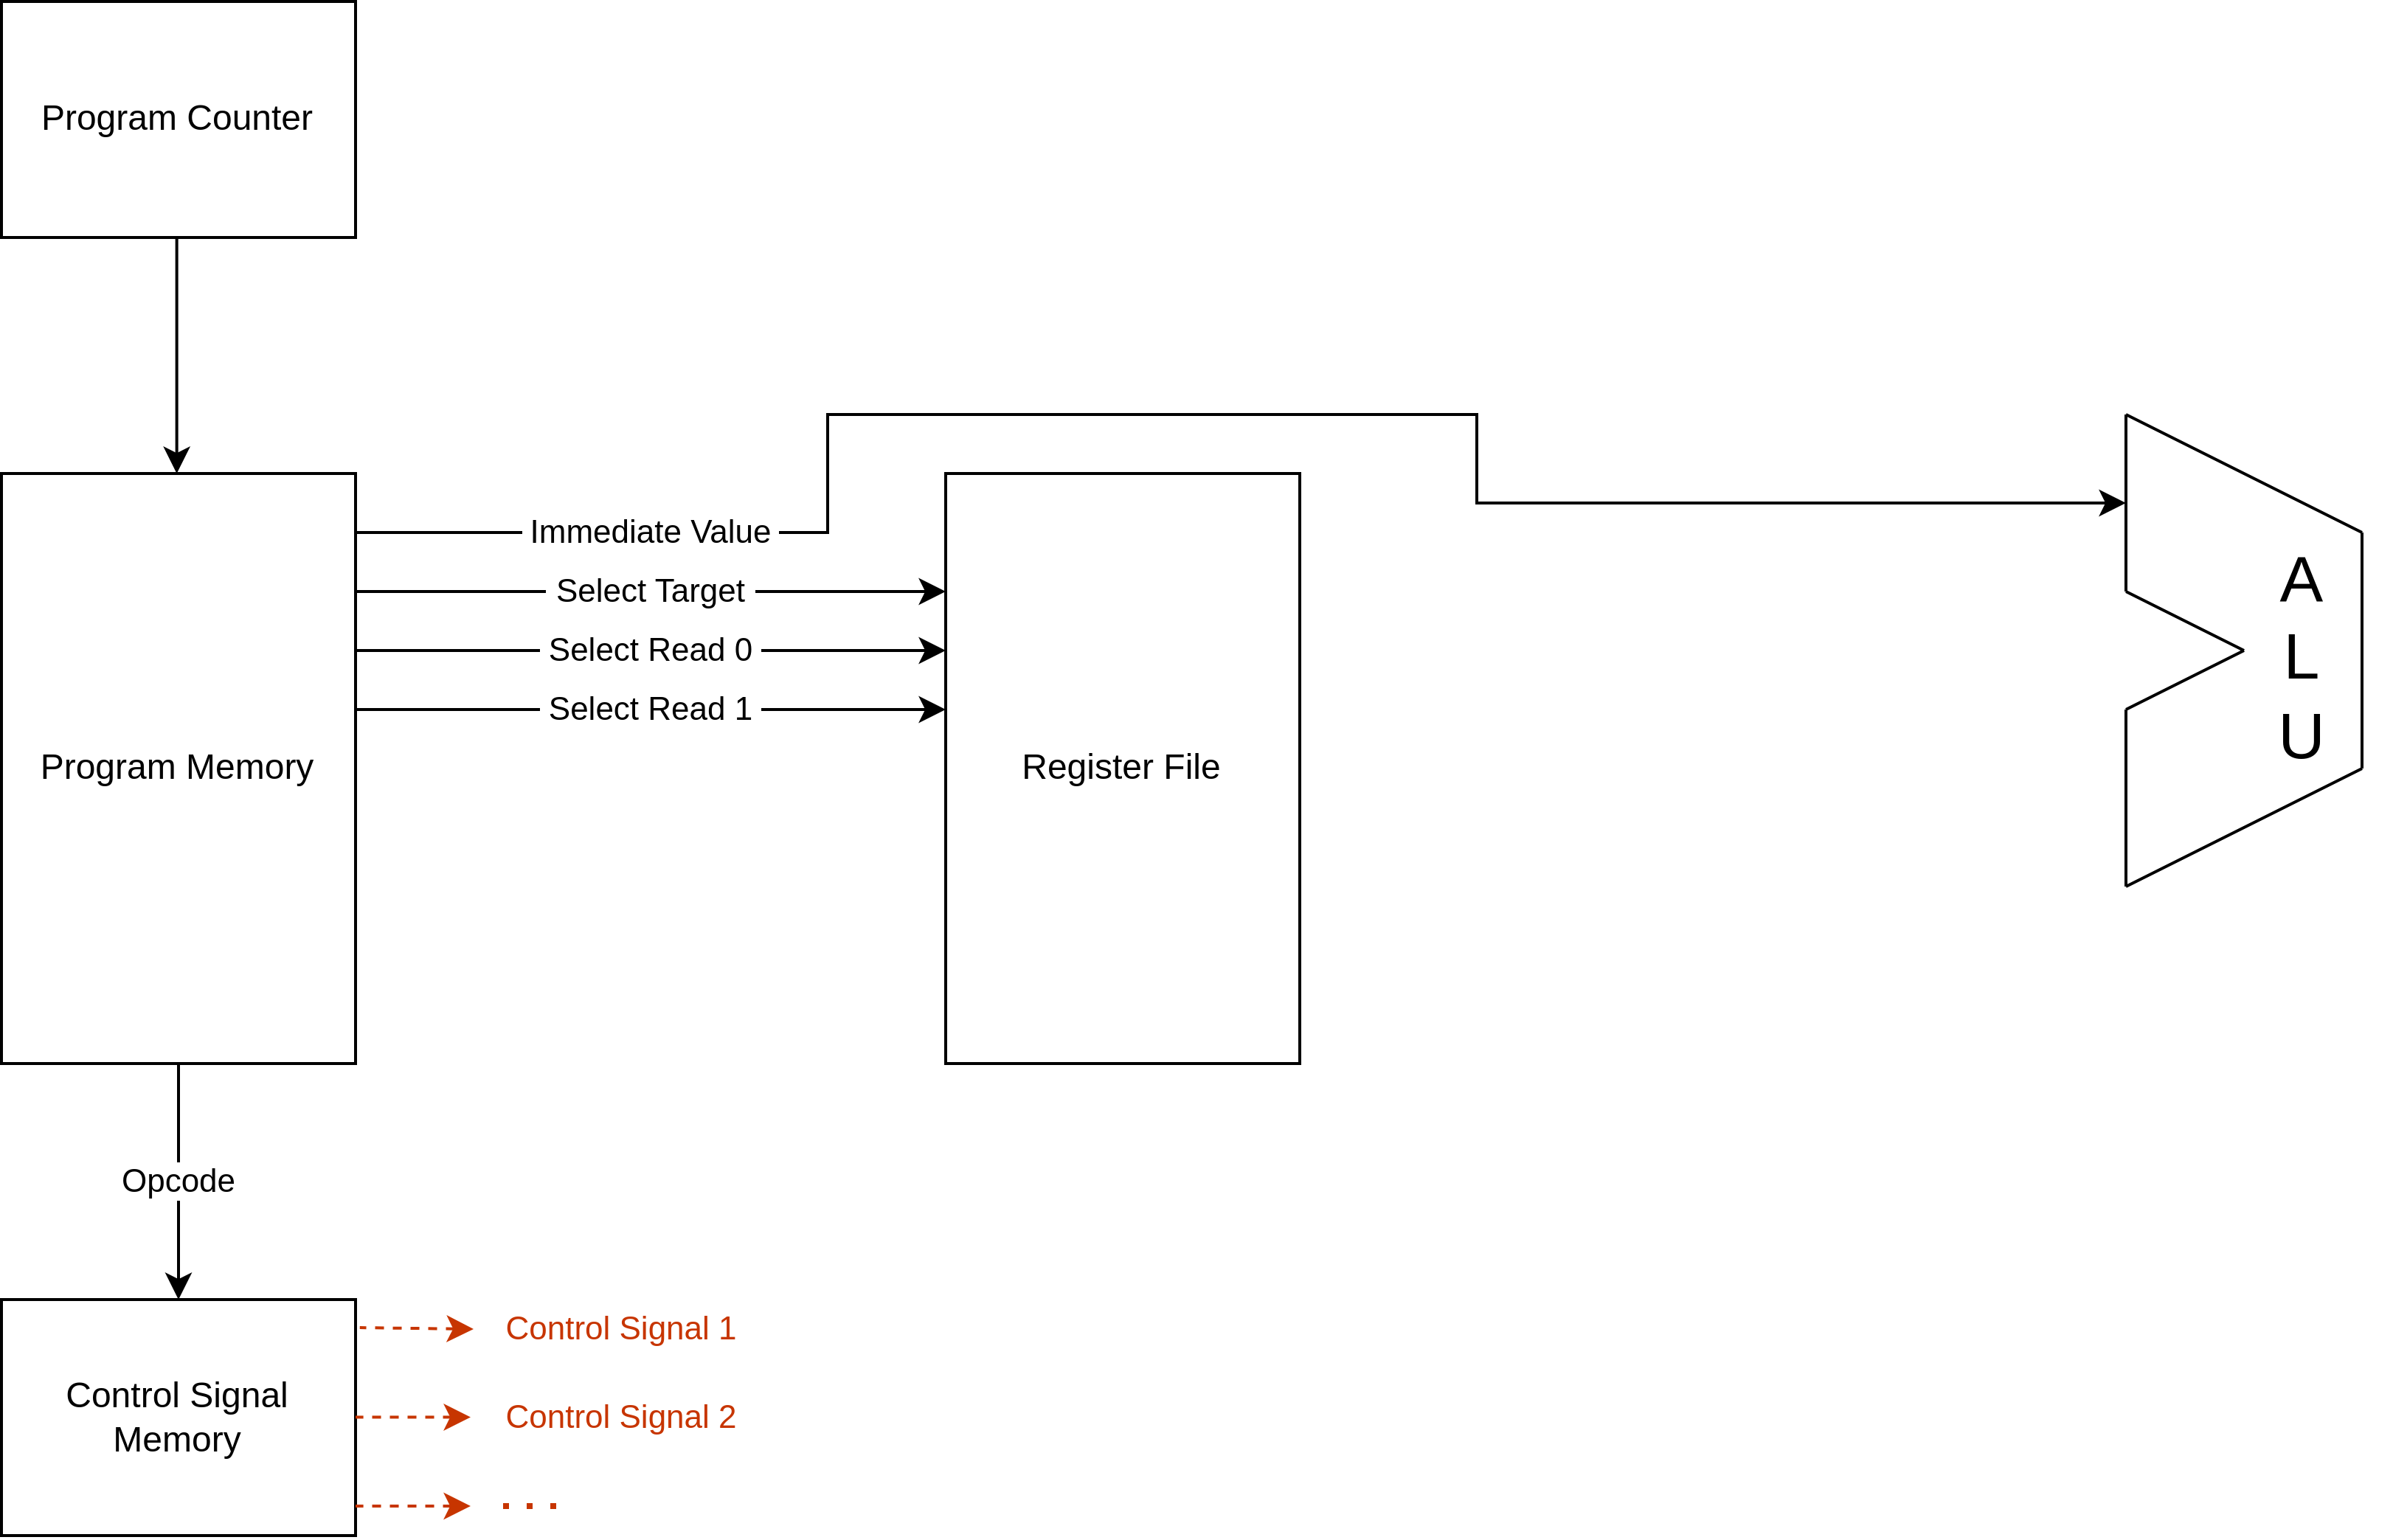
\includegraphics[width=1.0\textwidth]{images/drawio/datapath_operation_fields.png}  % Replace with your image file
    \caption{Datapath of instruction decoding. Solid black lines transport data, dotted red lines are control signals}
    \label{fig:implementation_interconnection_datapath_instruction_decoding}
\end{figure}

The register file must additionally receive two of the control signals to control when the relevant registers are updated. Likewise, the \ac{alu} receives control signals to choose which operation to perform and whether the operation needs a carry input. Two registers of the register file can be read and used as an input for \ac{alu} operations. However, the immediate value field of the instruction is already used as the first operand. For this reason, the first multiplexer is introduced. It switches the first operand between the immediate value and the first register being read from the register file. It also requires a control signal. From the register file, the contents of the flags register are constantly read, which are used as an input to the \ac{alu}, specifically the carry bit. The \ac{alu} outputs a result datum, as well as a set of flags, both of which are connected to the register file for writing back. \autoref{fig:implementation_interconnection_datapath_alu} shows the updated datapath after adding these connections.

\begin{figure}[h!]
    \centering
    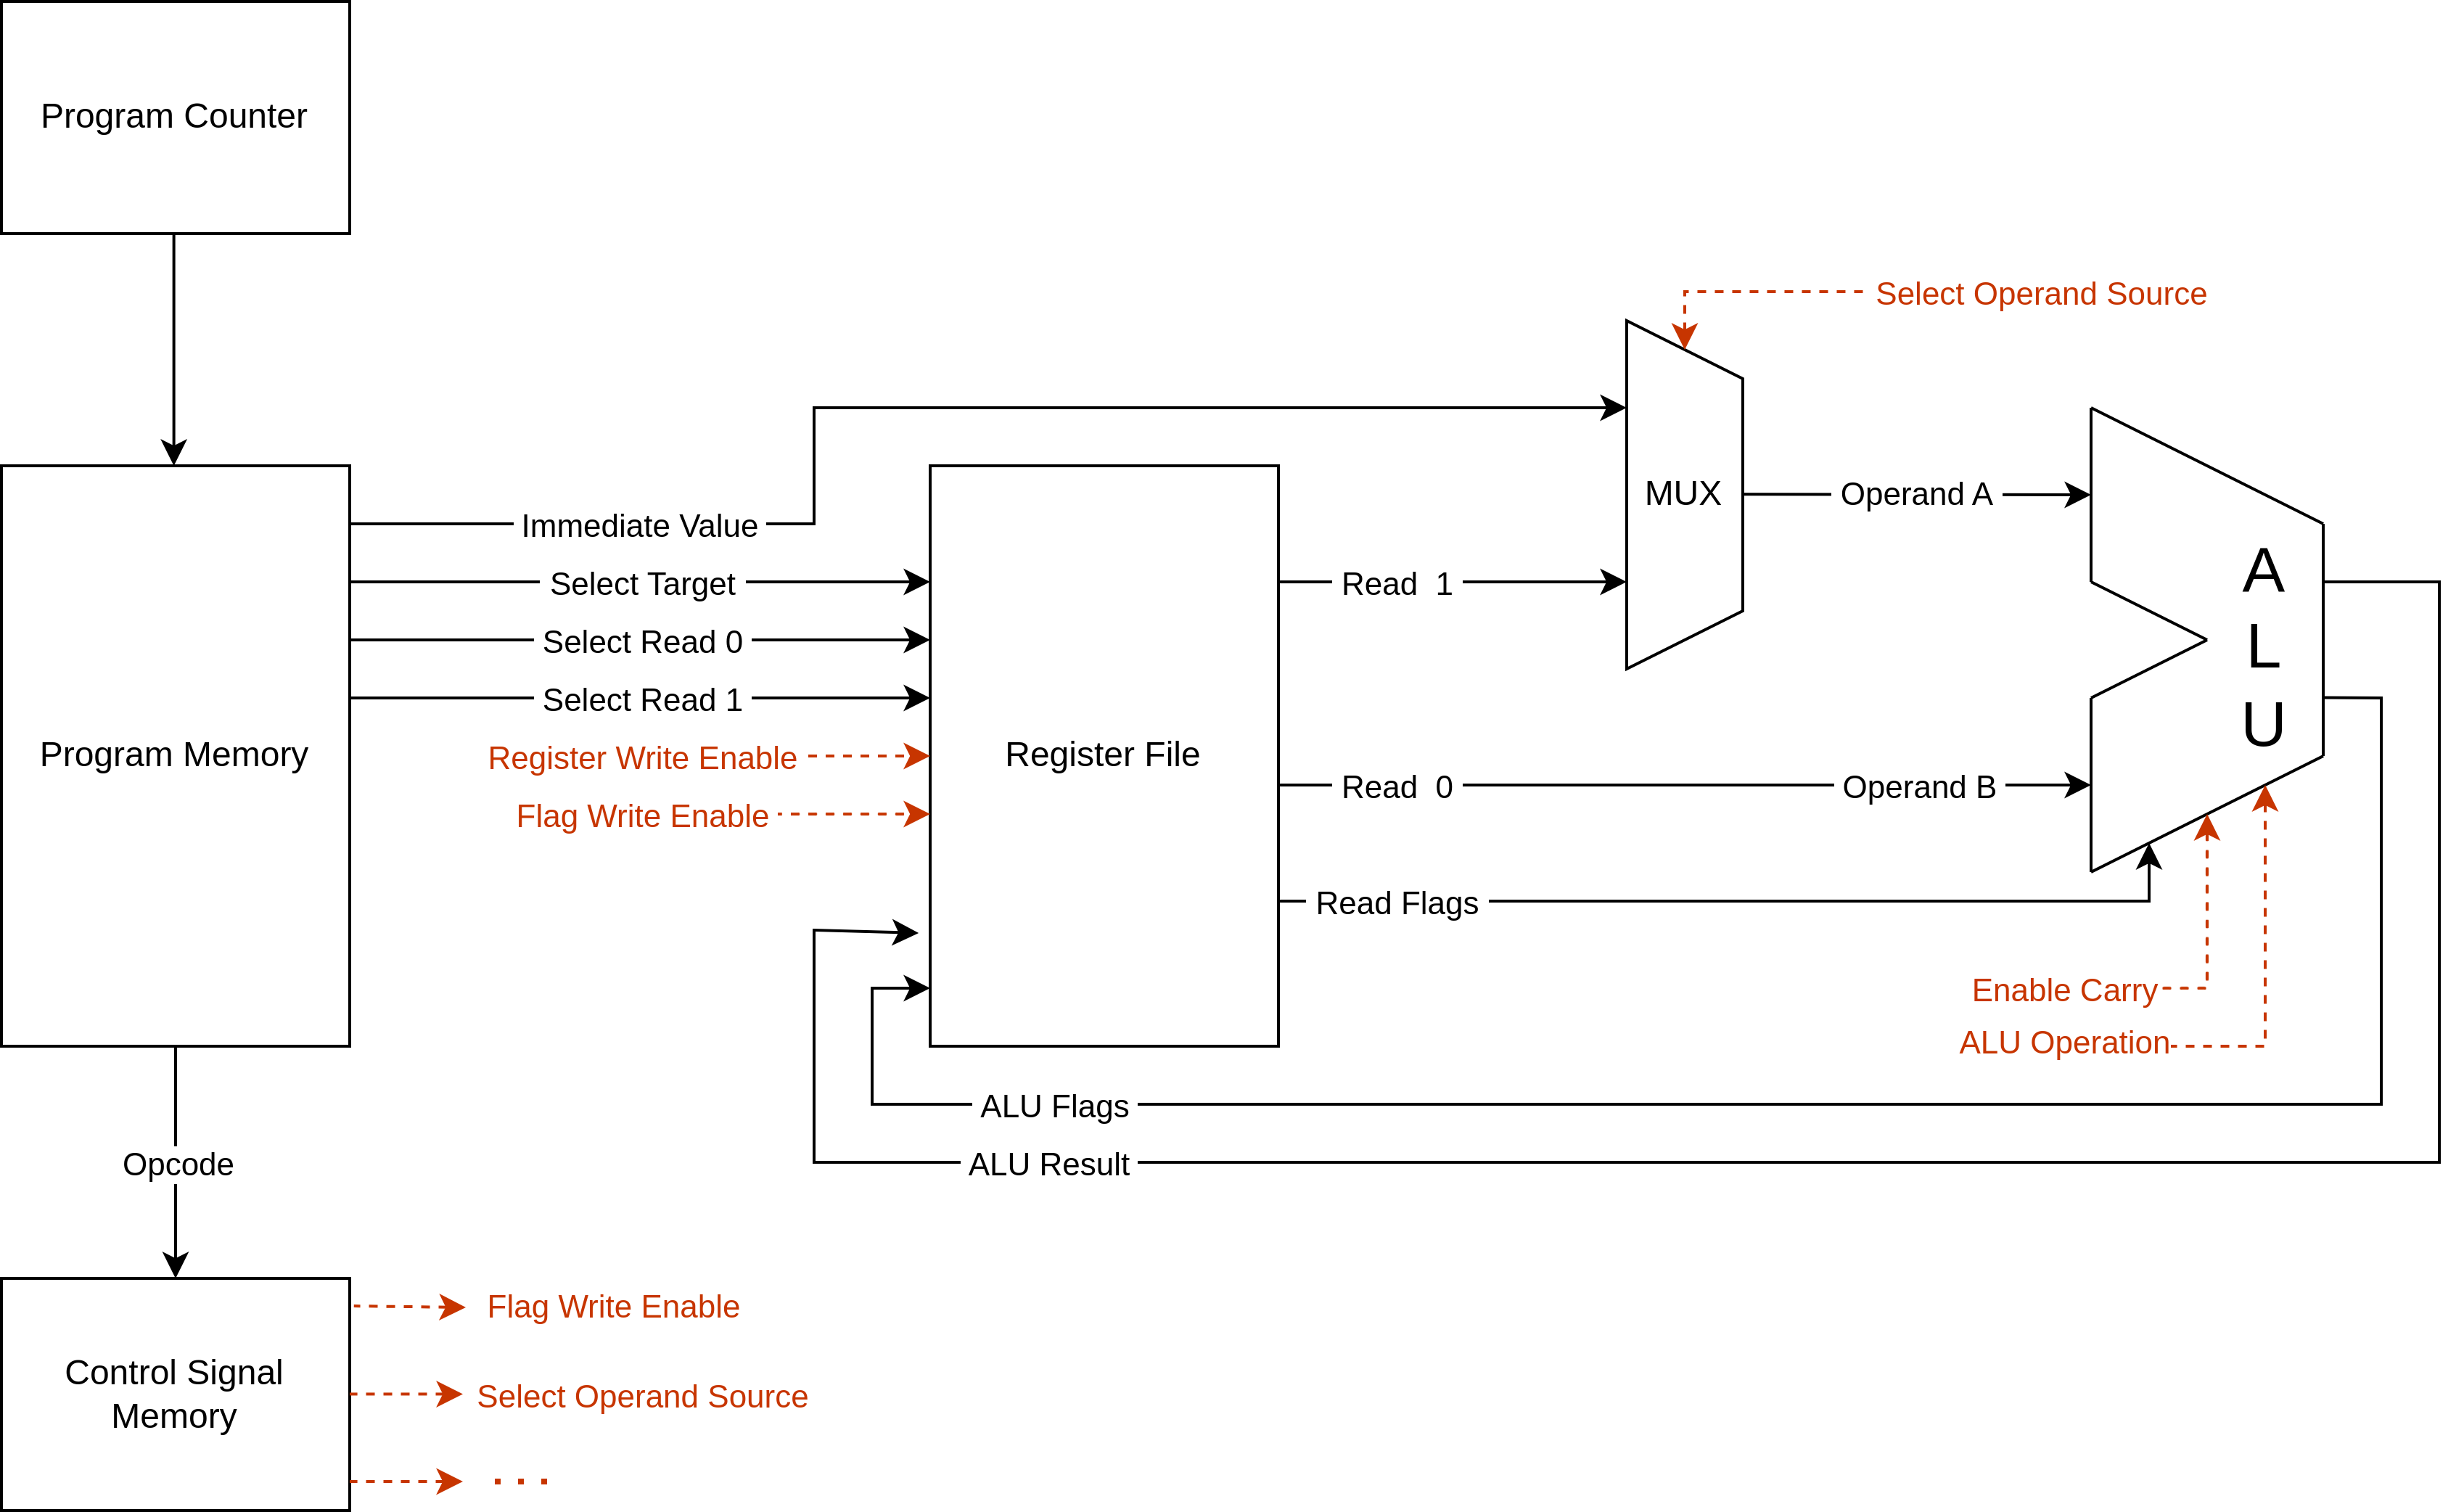
\includegraphics[width=1.0\textwidth]{images/drawio/datapath_operation_alu.png}  % Replace with your image file
    \caption{Datapath of instruction decoding and ALU. Solid black lines transport data, dotted red lines are control signals}
    \label{fig:implementation_interconnection_datapath_alu}
\end{figure}

In the current state, the contents of the program counter are static. However, it must be updated in order to progress program execution. The \ac{isa} specifies that it can either be incremented or overwritten by a branching instruction. Therefore, another multiplexer is introduced to choose between the two. Its output serves as the input to the program counter. The first multiplexer input is the output of an addition of the constant value 1 and the current program counter value. This realizes an incrementation, i.e the equivalent of sequentially loading the next instruction. The other input to the multiplexer is the branch address, which itself may also stem from two different sources. Therefore, it too is the output of another multiplexer. As defined in the \ac{isa}, the contents of registers \texttt{R6} and \texttt{R7} are constantly read and interpreted as a 16 bit address datum. This is the first source for the branch address. The second source is the 16 bit immediate value contained in the instruction. Both of these newly introduced multiplexers need a control signal. For selecting the source of the branch address, this is simply a control signal from the control unit. However, for selecting whether to branch or not, additional logic is necessary. This logical unit is described in more detail in \autoref{sec:branch_control_unit}. It receives two control signals, as well as the ``zero'' bit of the \ac{alu} flags result. It then computes and outputs the control signal for the branching multiplexer. All of these changes are shown in \autoref{fig:implementation_interconnection_datapath_pc}.
\begin{figure}[h!]
    \centering
    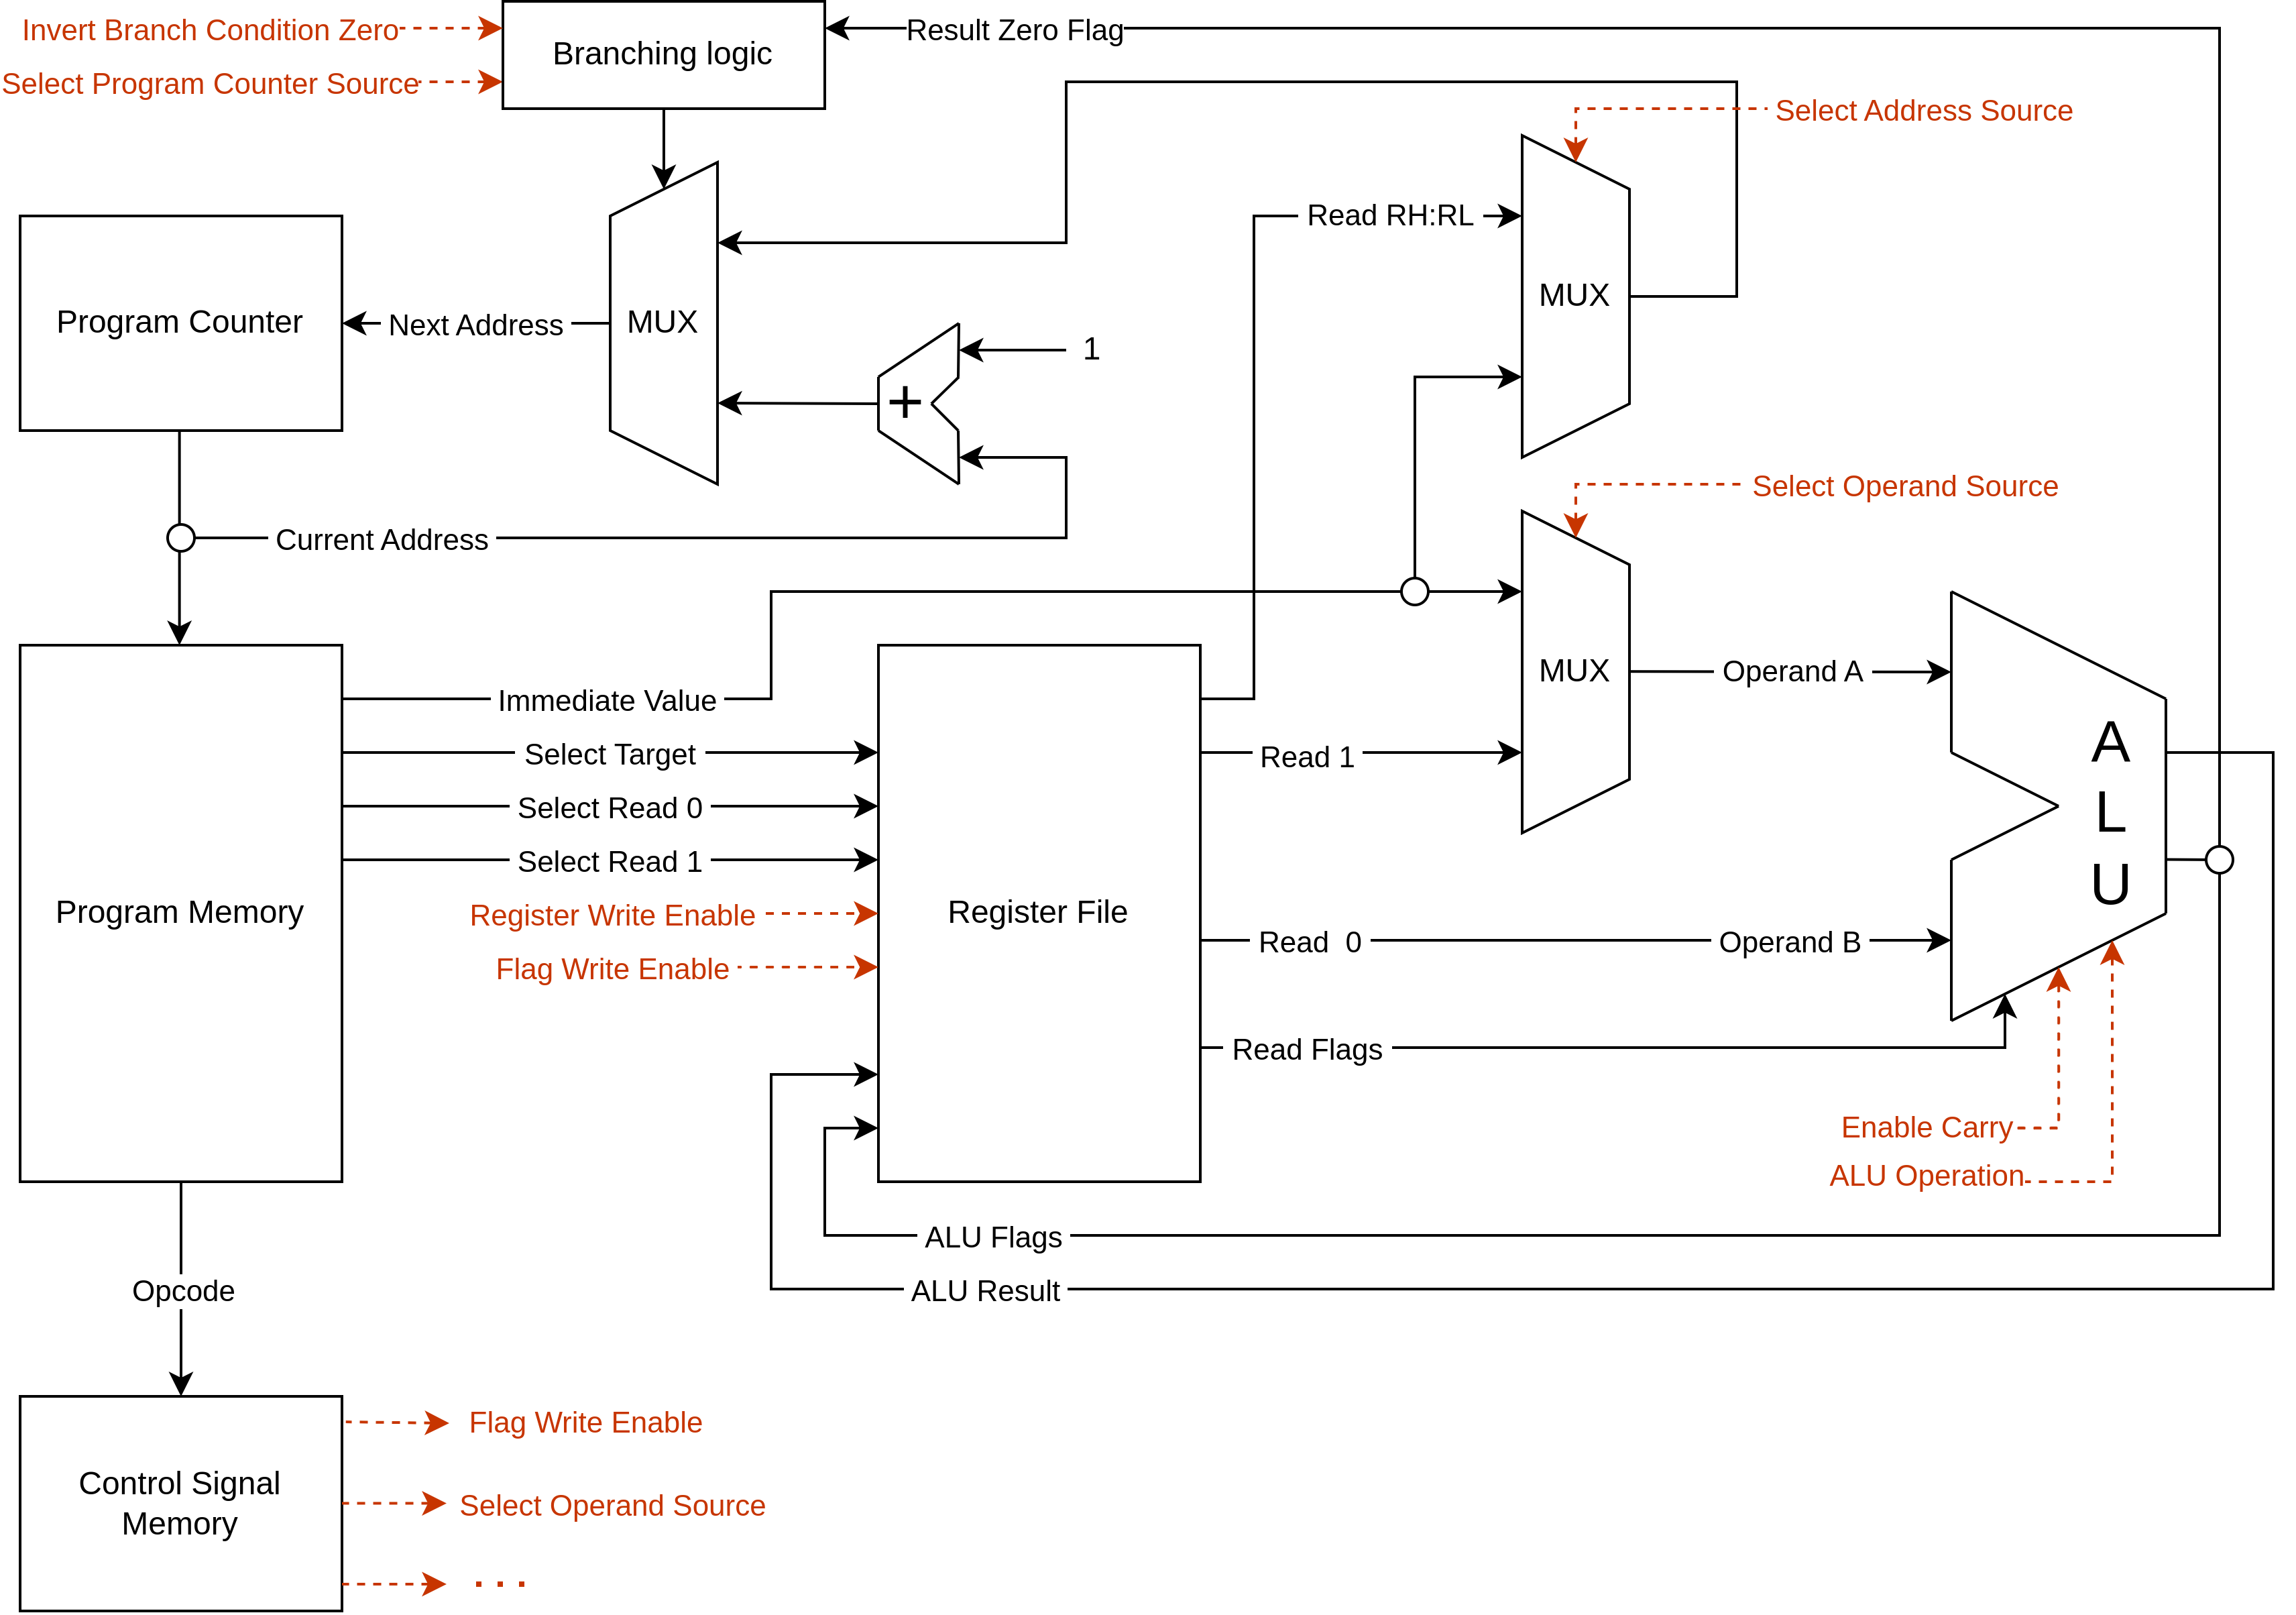
\includegraphics[width=1.0\textwidth]{images/drawio/datapath_operation_pc.png}  % Replace with your image file
    \caption{Datapath instruction decoding, ALU and program counter. Solid black lines transport data, dotted red lines are control signals}
    \label{fig:implementation_interconnection_datapath_pc}
\end{figure}

The last module to be connected is the working memory. It must receive an address input, for which the output of the branch address multiplexer is used. By doing so, memory access instructions can also use either an immediate address or the combination of registers \texttt{R6} and \texttt{R7}. The data input of the memory is connected to the output of reading the first selected register in the register file. The data output must be able to be written back to the register file. Since the data input of the register file is already connected to the output of the \ac{alu}, another multiplexer and control signal are introduced. In addition to that, the memory receives another pair of control signals to control when the programmer wants to read from or write to it. \autoref{fig:implementation_interconnection_datapath} shows the completed datapath diagram of a possible implementation of the \ac{ava} \ac{isa}. Clock signals are omitted for clarity of the datapath itself. There are 11 control signals in total. Since the \ac{alu} operation is encoded using three bits and the ``halt'' signal is omitted, there is a total of 15 individual control signal lines. This logical design diagram represents the register transfer level of the system.

\begin{figure}[h!]
    \centering
    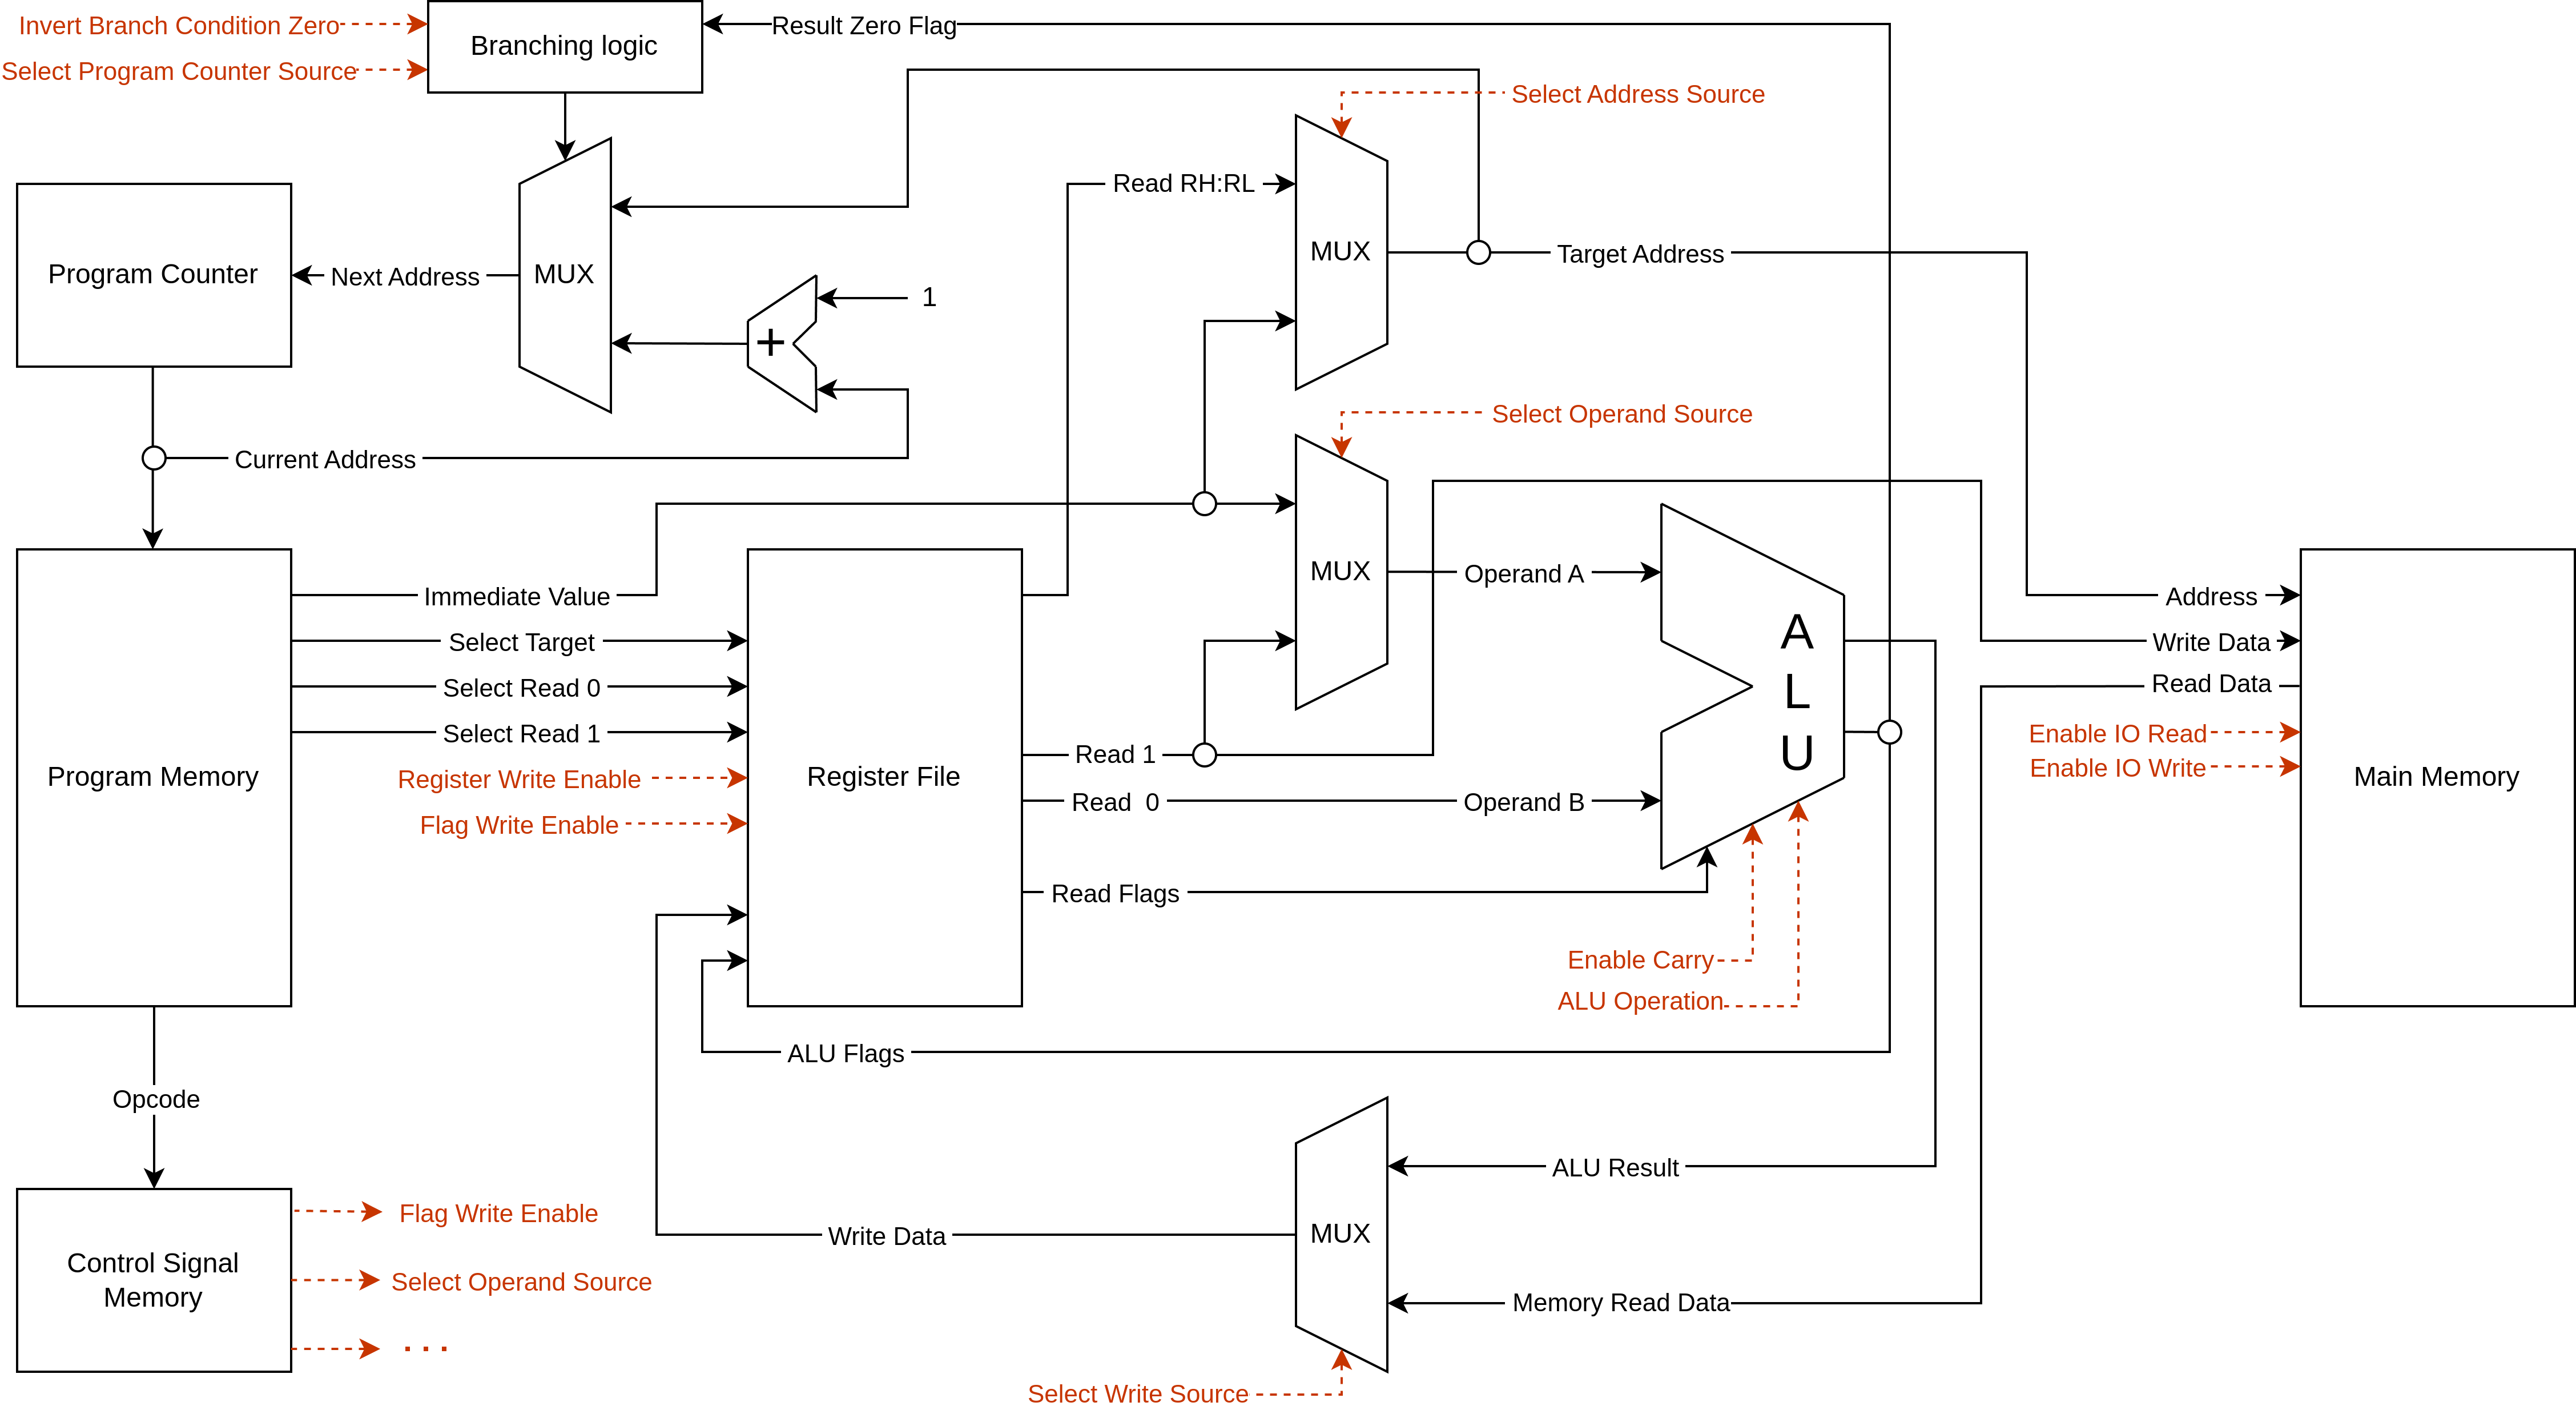
\includegraphics[width=1.0\textwidth]{images/drawio/datapath.png}  % Replace with your image file
    \caption{Datapath of an implementation of the \ac{ava} \ac{isa}. Solid black lines transport data, dotted red lines are control signals. Clock signals and external interfaces are omitted for clarity.}
    \label{fig:implementation_interconnection_datapath}
\end{figure}

